\documentclass[12pt,a4paper]{article}
\usepackage[polish]{babel}
\usepackage[utf8]{inputenc}
\usepackage[T1]{fontenc}

% dodatkowe pakiety
%\usepackage{enumerate}
\usepackage{listings}
%\lstloadlanguages{TeX}
\usepackage{amsmath}
\usepackage{fancyhdr}
%\usepackage{a4wide}
%\usepackage{pdfpages} %pdf
\usepackage[pdftex]{graphicx}
\usepackage{multirow}

\lstset{
  literate={ą}{{\k{a}}}1
           {ć}{{\'c}}1
           {ę}{{\k{e}}}1
           {ó}{{\'o}}1
           {ń}{{\'n}}1
           {ł}{{\l{}}}1
           {ś}{{\'s}}1
           {ź}{{\'z}}1
           {ż}{{\.z}}1
           {Ą}{{\k{A}}}1
           {Ć}{{\'C}}1
           {Ę}{{\k{E}}}1
           {Ó}{{\'O}}1
           {Ń}{{\'N}}1
           {Ł}{{\L{}}}1
           {Ś}{{\'S}}1
           {Ź}{{\'Z}}1
           {Ż}{{\.Z}}1
}

%\usepackage[colorlinks=true,urlcolor=blue,linkcolor=red,citecolor=green]{hyperref}
\usepackage[colorlinks=true,urlcolor=black,linkcolor=black,citecolor=black]{hyperref}


%marginesy
\usepackage{geometry}
\newgeometry{tmargin=2.5cm, bmargin=2.5cm, lmargin=2.5cm, rmargin=2.5cm}

%kropki przy numeracji
%\renewcommand\thesection{\arabic{section}.}
%\renewcommand\thesubsection{\thesection\arabic{subsection}.}

\author{Żaneta Błaszczuk, Jakub Porębski}
\title{Projektowanie tras biegowych w mieście}	
\date{12 stycznia 2015}

\pagestyle{fancy}
\fancyhead[R]{Żaneta Błaszczuk, Jakub Porębski}
\fancyhead[L]{Projektowanie tras biegowych w mieście} 		
\fancyfoot[C]{\thepage}

\begin{document}
\begin{titlepage}

\newcommand{\HRule}{\rule{\linewidth}{0.5mm}} % Defines a new command for the horizontal lines, change thickness here

\center % Center everything on the page
 
%----------------------------------------------------------------------------------------
%	HEADING SECTIONS
%----------------------------------------------------------------------------------------

\textsc{\LARGE Akademia Górniczo - Hutnicza}\\[1.5cm] % Name of your university/college
\textsc{\Large Wydział Elektrotechniki, Automatyki,\protect\\[-1mm] Informatyki i Inżynierii Biomedycznej}\\[0.5cm] % Major heading such as course name
\textsc{\large Matematyczne metody wspomagania decyzji}\\[0.5cm] % Minor heading such as course title

%----------------------------------------------------------------------------------------
%	TITLE SECTION
%----------------------------------------------------------------------------------------

\HRule \\[0.4cm]
{ \huge \bfseries Projektowanie tras biegowych w mieście zrealizowane z wykorzystanie algorytmu Tabu Search}\\[0.4cm] % Title of your document
\HRule \\[1.5cm]
 
%----------------------------------------------------------------------------------------
%	AUTHOR SECTION
%----------------------------------------------------------------------------------------

\begin{minipage}{0.4\textwidth}
\begin{flushleft} \large
\emph{Projekt zrealizowali:}\\
Żaneta \textsc{Błaszczuk} \\ % Your name
Jakub \textsc{Porębski}
\end{flushleft}
\end{minipage}
~
\begin{minipage}{0.5\textwidth} %w razie czego 0.4
\begin{flushright} \large
\emph{Prowadzący:} \\
Dr inż. Piotr \textsc{Kadłuczka} % Supervisor's Name
\end{flushright}
\end{minipage}\\[1cm]

% If you don't want a supervisor, uncomment the two lines below and remove the section above
%\Large \emph{Autor:}\\
%Jakub \textsc{Porębski}\\[3cm] % Your name

%----------------------------------------------------------------------------------------
%	DATE SECTION
%----------------------------------------------------------------------------------------


{\large 12 stycznia 2015}\\[1cm] % Date, change the \today to a set date if you want to be precise

%----------------------------------------------------------------------------------------
%	LOGO SECTION
%----------------------------------------------------------------------------------------



\includegraphics[height=50mm]{agh.jpg}%\\[1cm] % Include a department/university logo - this will require the graphicx package
 
%----------------------------------------------------------------------------------------

\vfill % Fill the rest of the page with whitespace

\end{titlepage}
\tableofcontents
\newpage

\section{Abstract}
Sprawozdanie piszemy w formie bezosobowej: wykonano, zrobiono, obliczono



\section{Opis problemu}
Podczas planowania trasy biegowej często nie chcemy dobiec do danego punktu najkrótszą możliwą drogą, lecz drogą o określonej długości. Jednocześnie jeżeli teren po którym biegamy jest pagórkowaty możemy unikać zmian wysokości, bądź wręcz przeciwnie ich oczekiwać. Równocześnie wiedząc o szkodliwości biegania po betonie możemy chcieć zminimalizować ilość dróg betonowych na naszej trasie.

\section{Parametry modelu}
Celem algorytmu jest znalezienie optymalnej trasy o długości najbardziej zbliżonej do zadanej przez użytkownika z uwzględnieniem parametru wysokości oraz ilości betonu na trasie biegu.

\subsection{Uproszczenia i uogólnienia}
W trakcie implementacji algorytmu przyjęto założenie, że badany graf jest grafem planarnym, który dobrze opisuje układ dróg w mieście. Algorytm przybliża długości dróg do linii prostych, nie uwzględniając zakrętów na trasie.
Równocześnie przyjęto, że atrakcyjność danej trasy zależy wyłącznie od różnicy wysokości na trasie oraz od ilości dróg asfaltowych na trasie.

\subsection{Parametry i zależności}
Głównymi parametrami trasy jest mapa krawędzi, po których może przebiegać trasa. Zawiera ona jednocześnie informacje o wysokości w każdym węźle grafu oraz o rodzaju nawierzchni.

Do parametrów algorytmu zaliczamy również zadaną przez użytkownika odległość orza preferencje własne dotyczące trasy.

\subsection{Postać rozwiązania}
Rozwiązaniem naszego problemu jest uporządkowana lista krawędzi grafu, która osiąga minimalną wartość funkcji celu.
\subsection{Funkcja celu}
Minimalizowano funkcję celu problemu poszukiwania optymalnej trasy biegowej, która wygląda następująco:
\begin{equation}
	f(d,h,b) = 
	w_1 \left|\overline{d} - \sum\limits_{i=1}^{n} d_{i} \right| + 
	w_2 \sum\limits_{i=1}^{n} \left|\overline{h} -  |h_{i}|\right| + 
	w_3 \left|\overline{b} - \dfrac{\sum\limits_{i=1}^{n} b_{i}}{n} \right|
\end{equation}

$d_i > 0$ -- długość i-tej krawędzi\\
$h_i$ -- różnica wysokości na i-tej krawędzi\\
$b_i$ -- rodzaj nawierzchni na i-tej krawędzi (0 -- nawierzchnia dobra, 1 -- nawierzchnia betonowa)\\
$\overline{d}$ -- zadana wartość drogi\\
$\overline{h}$ -- zadana wartość różnicy wysokości na każdej krawędzi\\
$\overline{b}$ -- zadana ilość dróg o nawierzchni betonowej w \% \\
$w_1, w_2, w_3$ -- wagi dobierane przez użytkownika

\subsection{Ograniczenia}

\section{Implementacja algorytmu}
Algorytm Taboo Search
\subsection{Postać danych}
Dane w trakcie wykonywania algorytmu są przechowywane w kilku macierzach przyległości. Program w celu rozpoczęcia pracy potrzebuje 7 plików wejściowych z kolejnymi strukturami danych:
\begin{enumerate}
\item Współrzędne wierzchołków
	\begin{itemize}
	\item rozszerzenie: .xy
	\item Pierwsza linia: h w -- wysokość i szerokość grafu
	\item Kolejne linie: wartości współrzędnych X Y każdego punktu
	\end{itemize}
\item Krawędzie
	\begin{itemize}
	\item rozszerzenie: .kr
	\item Pierwsza linia: n -- liczba krawędzi
	\item Kolejne linie: X1, Y1, X2, Y2
	\end{itemize}
\item Macierz przyległości\\
Macierz kwadratowa przeskalowanych odległości między wierzchołkami
	\begin{itemize}
	\item rozszerzenie: .txt
	\item Pierwsza linia: h*w -- liczba wierzchołków
	\item Kolejne linie: wartości kolejnych komórek, 0 oznacza nieskończoność
	\end{itemize}
\item Lista wysokości
	\begin{itemize}
	\item rozszerzenie: .wys
	\item Pierwsza linia: min max - minimalna i maksymalna wysokość
	\item Kolejne linie: wysokości kolejnych wierzchołków
	\end{itemize}
\item Macierz wysokości
	\begin{itemize}
	\item rozszerzenie: .mwys
	\item Pierwsza linia: h*w -- liczba wierzchołków
	\item Kolejne linie: jak w macierzy przyległości. Zawiera różnicę między dwoma łączonymi wierzchołkami
	\end{itemize}
\item Lista betonowości
	\begin{itemize}
	\item rozszerzenie: .bet
	\item Pierwsza linia: h*w -- liczba krawędzi
	\item Kolejne linie: wartości, 0 oznacza brak betonu, 1 to beton (bardzo nie atrakcyjne)
	\end{itemize}
\item Macierz wysokości
	\begin{itemize}
	\item rozszerzenie: .mbet
	\item Pierwsza linia: h*w -- liczba wierzchołków
	\item Kolejne linie: jak w macierzy przyległości. Symetryczna, nieujemna
	\end{itemize}				
\end{enumerate}

\subsection{Struktury danych}
\subsubsection{Klasa graph}
Klasa graph opisuje w pełni wszystkie połączenia i wierzchołki w badanym grafie.

\subsection{Interface użytkownika}
\begin{figure}[!h]
	\centering
	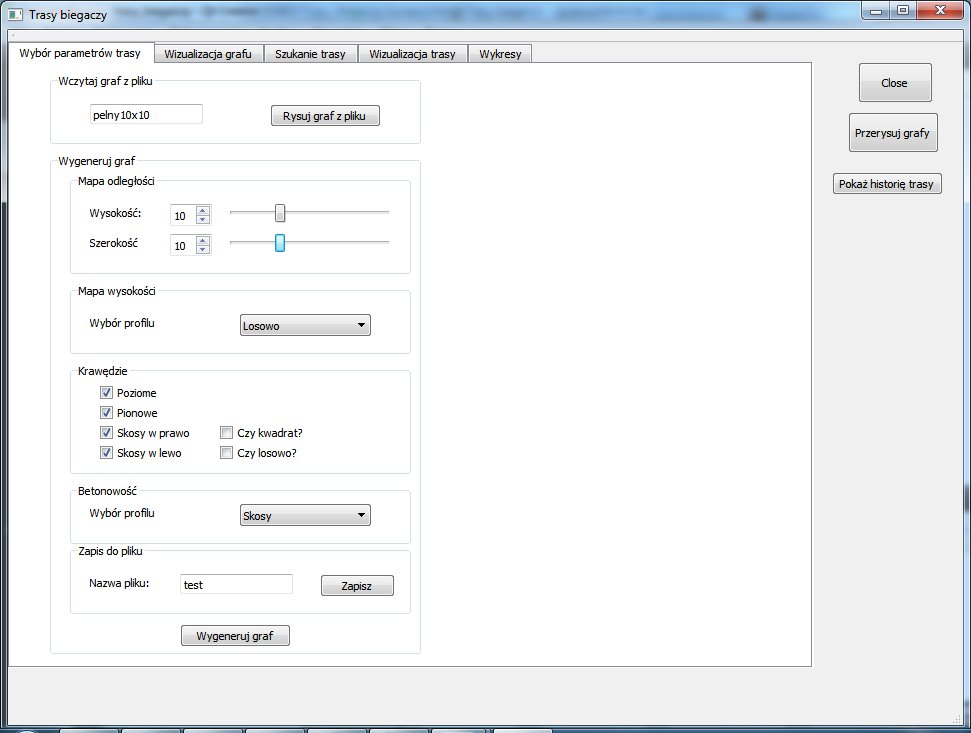
\includegraphics[height=110mm]{./ilustracje/screen1.png}
\end{figure}

\section{Testowanie algorytmu}
\subsection{Test 1}

\section{Analiza efektywności}
\section{Podsumowanie}



\end{document}
